% This is lnbip.tex the demonstration file of the LaTeX macro package for
% Lecture Notes in Business Information Processing from Springer-Verlag.
% It serves as a template for authors as well.
% version 1.0 for LaTeX2e
%
\documentclass[lnbip]{svmultln}
%
\usepackage{makeidx}  % allows for indexgeneration
% \makeindex          % be prepared for an author index
\usepackage[numbers]{natbib}
\usepackage{graphicx}
\usepackage{framed}


%
\begin{document}
%
\mainmatter              % start of the contribution
%
\title{Towards Quality-Driven SOA Systems Refactoring through Planning}
%
\titlerunning{Towards Quality-Driven SOA Systems Refactoring through Planning}  % abbreviated title (for running head)
%                                     also used for the TOC unless
%                                     \toctitle is used
%
\author{Mathieu Nayrolles\inst{1} \and Eric Beaudry\inst{2}
Naouel Moha\inst{2} \and Petko Valtchev\inst{2} \and Abdelwahab Hamou-Lhadj\inst{1} }
%
\authorrunning{Mathieu Nayrolles et al.}   % abbreviated author list (for running head)
%
\institute{SBA Research Lab, ECE Department, Concordia University, Montréal, Canada\\
\email{m_nayrol@encs.concordia.ca, abdelw@concordia.ca},\\ 
\and
D\'epartement d`informatique, Universit\'e du Qu\'ebec à Montr\'eal, Canada\\
\email{{eric.beaudy, naouel.moha, petko.valtchev}@uqam.ca
}}

\maketitle              % typeset the title of the contribution
% \index{Ekeland, Ivar} % entries for the author index
% \index{Temam, Roger}  % of the whole volume
% \index{Dean, Jeffrey}

\begin{abstract}        % give a summary of your paper
Service Based Systems (SBSs), like other software systems, evolve due to changes in both user requirements and execution contexts. Continuous evolution could easily deteriorate the design and reduce the Quality of Service (QoS) of SBSs and may result in poor design solutions, commonly known as SOA (Service Oriented Architecture) antipatterns. SOA antipatterns lead to a reduced maintainability and re-usability of SBSs. It is therefore critical to be able to detect and remove them to ensure the architectural quality of the software during its lifetime. In this paper, we present a novel approach named SOMAD-R (Service Oriented Mining for Antipattern Detection-Refactoring) which allows the refactoring of SOA antipatterns by building on a previously published tool named SOMAD (Service Oriented Mining for Antipattern Detection). SOMAD-R combines planning solving techniques and SOMAD detection algorithms to enable antipatterns driven refactoring of SBSs. As a first step towards refactoring antipatterns for SBSs, we successfully applied SOMAD-R to HomeAutomation, a SCA (Service Component Architecture) application and we removed three antipatterns (out of five) while improving application’ performance by 32\%.
%                         please supply keywords within your abstract
\keywords {SOA Antipatterns, Quality-driven refactoring, SOA refactoring, Services orchestration, SOA planning
}
\end{abstract}
%
\section{Introduction}
%

Service Based Systems (SBSs) are composed of ready-made services that are accessed through the Internet \cite{Erl}. Services are autonomous, interoperable, and reusable software units that can be implemented using a wide range of technologies like Web Services, REST (REpresentational State Transfer), or SCA (Service Component Architecture, on the top of SOA.). Most of the world largest computational platforms such as Amazon, Paypal, and eBay, for example, represent large-scale SBSs. Such systems are complex--they may generate massive flows of communication between services--and highly dynamic: services appear, disappear, and can be modified over time. 

The constant evolution of SBSs can easily deteriorate the overall architecture of the system, causing architectural defects, known as SOA antipatterns \cite{Palma}.
An antipattern is the opposite of a design pattern. While design patterns should be followed to create more maintainable and reusable systems~\cite{wolfgang1994design}, antipatterns should be avoided since they have a negative impact on the maintenance and reusability of SBSs. 

Considering that SOA antipatterns reduce the capability to evolve, reuse, and understand these systems, it is thus important to detect and remove them. However, techniques to master the evolution of complex software systems are often based on historical change logs analyses rather than potentially harmful architectural impacts. 

In this paper, we propose a new and innovative approach named SOMAD-R (Service Oriented Mining For Antipattern Detection and Refactoring). This approach is an evolution of another approach--we introduced in a previous contribution \cite{Nayrolles2013a}--named SOMAD, which detects SOA antipatterns in execution traces produced by SBSs. Our approach goal is to leverage SOMAD’s detection to improve the overall software quality by means of refactoring.

Numerous approaches and tools have been proposed in the area of the detection and correction of antipatterns in object-oriented (OO) systems (for example, \cite{kessentini2011design, erni1996applying, fenton1998software, Moha2010, opdyke1992refactoring}). However, the dynamic nature of SBSs and the non-availability of the implementation of their interfaces do not allow to apply these approaches. Moreover, SOA focuses on services as first-class entities whereas OO focuses on object interactions, which are at the lower level of granularity.

To re-orchestrate the services’ communications while keeping the system working, we use automated planning techniques. Automated planning techniques will generate a plan to reach an objective by using a set of actions that have effects and preconditions. We use SOMAD reverse-engineering capacities to extract the set of actions that the system under study  exposes and we generate plans that keep the system behaviour while proposing a better orchestration. The generated plans are then submitted to SOMAD in order to assess their quality in terms of SOA antipatterns.  While there are time and memory available the iterative process of generating a plan and assess the amount of SOA antipattern detected by SOMAD continues. 

 In order to validate the effectiveness of our approach, we applied it to the HomeAutomation SCA (Service Component Architecture) system. HomeAutomation targets the domotic control of elderly citizens' houses to ease the work of  doctors and nurses. On HomeAutomation, we performed the refactoring of the system and reduced the number of instances of antipatterns from five  to two. Also, as a proof of the pertinence of our approach, the needed time to reach the same system state as in the initial services' orchestration has been reduced by 32\%.
 
The main contribution of this paper is an approach that allows enhancing the overall quality of a SBS by refactoring its antipatterns. 

The remainder of this paper is organized as follows. Section II presents related work in the area of SOA antipattern detection and quality-driven software refactoring, followed by related work on service oriented planning. In Section III, we introduce background information on SOMAD and service orchestration to ease the reading of this paper. In Section IV, we showcase our approach in details while Section V presents our experimental. Finally, we provide some concluding remarks in Section VI.


\section{Related Works}

In this section, we present studies closely related to refactoring antipatterns in the object-oriented (OO) world , QoS based orchestration and services orchestration by planing in SBSs. 

\subsection{Quality based refactoring of objects systems}
In the OO paradigm, two main trends arise for refactoring design deffects. In the first trend, researches first detect antipatterns and then remove them by applying refactoring technique. To date, they explore a wide-range of technology to do so such as FCA \cite{moha2008using}, RCA \cite{moha2008refactorings}, model transformation \cite{moha2009generic}, metric based \cite{erni1996applying, fenton1998software, Moha2010} and rules based \cite{opdyke1992refactoring}.
The second trend contains approaches that do not detect antipatterns per se but elements to modify in order to improve the overall quality of the system as in \cite{o2008search}.

Although some of these approaches and tools could be re-used for SOA, especially the metric based by using SOA metrics \cite{Nayrolles,Palma, demange2013,  Nayrolles2013a}, but it is difficult to define threshold values for metrics. Moreover, how to refactor SOA antipatterns, even manually, have only been explored based on strict use cases \cite{zhu2009refactoring, kim2007service}. Finally, those approaches and techniques have been conceptualized and improved over the years to fit the OO paradigm and it will not be trivial to adapt them to the SOA paradigm. 

\subsection{QoS Based Service Composition}

While not oriented towards antipatterns refactoring, a significant effort has been made to propose  QoS-oriented  approaches for service composition. These approaches can be separated into two distinct categories as proposed by \cite{Pejman2012}. Methods based on genetic algorithm \cite{canfora2005approach, zeng2003quality} (and related \cite{xu2008towards, ming2007approach}) and methods based on non-evolutionary algorithms such as dynamic programming \cite{yu2005service}.  All these approaches and techniques have in common that they try to maximize the availability and reliability while minimizing the cost and response time of the composed system. Although availability, reliability and response time are metrics to detect antipatterns, they did not have this level of abstraction and only target the Quality of Service. Quite the opposite, our approach deal with software quality as a vector to improve maintenance, re-usability and evolution of the system while keeping QoS in mind.

\subsection{Service Composition By Planning}

In service composition or orchestration by planning, several works have been proposed to compose stateless \cite{narayanan2002simulation}, statefull \cite{berardi2005composition, marconi2006specifying} and even coordinated asynchronous statefull services \cite{pistore2005automated, bertoli2009continuous}.  However, these works focus on how many goals, e.g. how many services, they are able to aggregate/orchestrate in a minimum amount of time using advanced planning techniques and algorithms. Moreover, most of these approaches will compose a super-service containing all composed services and expose the newly created service which is, by definition, a multi-service antipattern and/or even a sandpile \cite{Palma}.


\section{Background}

In this section, we provide some preliminaries to ease the reading of further sections. We first present SOMAD, the approach upon which we build SOMAD-R. Then, we present the planning domain and the SOA-planning or orchestration. 


\subsection{The SOMAD Approach\label{somad}}

SOMAD relies on execution traces produced by SBSs in order to detect antipatterns. To achieve this, SOMAD uses data mining techniques. It discovers antipatterns by first extracting associations between services as expressed in the execution traces of an SBS. To that end, we apply a specific variant of the association rule mining task based on sequences and episodes \cite{Mannila1997}. In our case, the sequences represent services or, alternatively, method calls. Further, we filter these generated association rules by means of a suite of dedicated metrics. SOMAD includes the following three main steps.

\subsubsection{Specification SOA antipatterns:}

After a careful analysis of the SOA antipattern textual description, we create rule cards for six different antipatterns; Multi-Service, Tiny Service, Chatty Service, Knot Service, BottleNeck Service and Chain service. Rule cards are combinations of height different metrics dedicated to SOA antipattern detection. The definition of SOA antipatterns and metrics definition have been specified in \cite{Palma} and \cite{Nayrolles2013a}, respectively. The rule card are combined to automatically create detection algorithms using java templates \cite{Nayrolles}.
%
%
%\begin{table}
%\caption{List of SOA Antipatterns \cite{Moha} \label{tab:List-of-SOA}}
%\begin{tabular*}{12cm}{@{\extracolsep{\fill}}p{12cm}}
%\tabularnewline
%\hline 
%\noalign{\vskip0.3cm}
%\textbf{Multi-Service}, \textit{a.k.a} God Object corresponds to a service
%that implements a \textbf{multitude of methods} related to different
%business and technical abstractions. This aggregate too much into
%a single service, such a service is not easily reusable because of
%the \textbf{low cohesion} of its methods and is often unavailable
%to end-users because of its overload, which may induce a high response
%time \cite{Dudney2003}.\tabularnewline
%\noalign{\vskip0.2cm}
%\textbf{Tiny Service} is a small service with\textbf{ few methods}, which only
%implements part of an abstraction. Such service often requires \textbf{several
%coupled services} to be used together, resulting in higher development
%complexity and reduced usability. In the extreme case, a Tiny Service
%will be limited to \textbf{one method}, resulting in many services
%that implement an overall set of requirements \cite{Dudney2003}.\tabularnewline
%\noalign{\vskip0.2cm}
%\textbf{Chatty Service} corresponds to a set of services that exchange a \textbf{lot
%of small data} of primitive types. The Chatty Service is also characterized
%by a\textbf{ high number of method invocations}. Chatty Service chats
%a lot with each other \cite{Dudney2003}.\tabularnewline
%\noalign{\vskip0.2cm}
%\textbf{The Knot} is a \textbf{set of very} \textbf{low cohesive} services,
%which are tightly coupled. These services are thus less reusable.
%Due to this complex architecture, the availability of these services
%can be low, and their response time high \cite{Rotem-Gal-Oz2012}.\tabularnewline
%\noalign{\vskip0.2cm}
%\textbf{Bottleneck Service} is a service that is \textbf{highly used} by other
%services or clients. It has a \textbf{high incoming and outgoing coupling}.
%Its response time can be higher because it may be used by too many external
%clients, for which clients may need to wait to get access to the service.
%Moreover, its availability may also be low due to the traffic.\tabularnewline
%\noalign{\vskip0.2cm}
%\textbf{Service Chain}, a.k.a. Message Chain in OO systems, corresponds
%to a \textbf{chain of services}. The Service Chain appears when clients
%request \textbf{consecutive service invocations} to fulfill their
%goals. This kind of \textbf{dependency chain} reflects the action
%of invocation in a transitive manner.
%\tabularnewline
%\tabularnewline
%\hline 
%\vspace{.1cm}
%\end{tabular*}\end{table}

\subsubsection{Mining Sequential association rules}

In the data-mining field, Association Rule Mining (ARM) is a well-established method for discovering co-occurences between attributes in the objects of a large data set \cite{Gregory1991}. Plain association rules have the form X $\rightarrow$ Y, where X and Y are sets of descriptors. While plain association rules could provide interesting information, we decide to use a variant named Sequential Association Rules to preserve the sequences of service/method calls. Applying this technique on execution traces files identify interesting relations between services like: \textit{ServiceA}, \textit{ServiceB} \ implies\  \textit{ServiceC}
meaning that if services A and B appear, there is a high probability for C to appear in the same sequence of service calls.

\subsubsection{Detection of SOA Antipatterns:}

This step consists of applying the detection algorithms generated in Step 1 on the sequential association rules mined in Step 2. At the end of this step, services in the SBS suspected to be involved in an antipattern are identified.

Finally, the efficiency of SOMAD has been proved on two different systems named HomeAutomation and FraSCAti. The precision was 90.1\% and 94.44\% for HomeAutomation and FraSCAti respectively.

\subsection{Automated Planning for SOA}

Automated planning is a branch of Artificial Intelligence (AI) aiming to transform an environment on a given initial state to an environment that satisfies given goal(s) using a set of actions \cite{ghallab2004automated}. Each action have  effect(s) on the environment and might require pre-condition(s) to be executed. A planning problem takes place in a state transition system defined by:

\begin{equation}
\sum  = (S, A, E, \gamma)
\end{equation}

Where S, A, E represent the states, actions and events, respectively and $\gamma$ represents the state-transition function :

\begin{equation}
\gamma: S * (A \cup E)
\end{equation}

The solution of the planning problem will decide what actions to use to achieve the set of goal(s). The required complexity to solve a planning problem can be much more than NP-Complete or even undecidable. 
 A classical planning problem takes place in a finite, fully observable, deterministic, static system where goals can be reached with sequential plans and implicit time. This said, to solve a classical planning problem we have to find a sequence of actions $(a1, a2, ... , an)$ that produces a sequence of state transitions $(s1, s2, ..., sn)$ where $sn$ satisfies our goals. 

When applied to SOA, planning is often referred to as service orchestration. The complexity of manually orchestrating thousands of services participating in complex business logic led the community to use planning algorithms and techniques. However, techniques related to classical planning cannot be used as is. Indeed, in a SOA environment the system is not fully observable (inside logic of services are unknown), not always deterministic (services output can change overtime) and dynamic (services can be added or removed at any time). Despite these challenges, several works have been done and succeed to orchestrate services with conservative hypothesis. For example, they assume that the services outputs are deterministic and the environment static in a sense that every collaborating services and their actions are known beforehand. 

	In our study, we not only target the orchestration of services but a qualitative re-orchestration of services in terms of SOA antipatterns. Furthermore, we do not know what are the possible actions as we deduct them from SOMAD reverse engineering of a running SBS and not from the specification as previous studies. Consequently, we try to construct qualitative plans with a sub-set of the actions provided by the system. Depending on how long SOMAD observed the targeted SBS and how complete the utilisation of SBS is, the sub-set size will vary.

\section{The SOMAD-R Approach}

SOMAD-R is a complete approach which supports the refactoring of SOA systems in order to improve their conceptual quality in terms of SOA antipatterns. SOMAD-R is composed of three main steps and is depicted in Figure \ref{fig:appraoch}. The first step uses SOMAD to reverse-engineer the targeted system and provide the services suspected to be involved in antipatterns. The second step builds and resolves a planning problem with the aim of reaching all the services previously consumed while re-orchestrating the order of calls in order to reduce the amount of antipatterns. Finally, the last step receives the solution proposed by the second step and send the plan to SOMAD for it to assess the quality of the solution. We iterate over these three steps until we cannot improve the solution anymore or total consumption of resources.


\begin{figure}
    \centering
	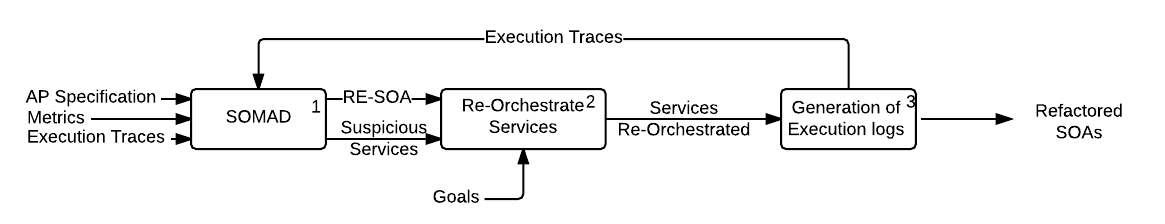
\includegraphics[width=\textwidth]{approach.png}
 	\caption{The SOMAD-R approach}
    \label{fig:appraoch}
\end{figure}


\subsection{SOMAD Antipattern Detection}

The first step consists in feeding SOMAD with the antipatterns specification, the metrics and the executions traces of a given SOAs as explained in section \ref{somad} and in \cite{Nayrolles2013a}. 

Figure \ref{fig:traces} presents the kind of execution traces that SOMAD requires to perform its detection. Every trace contains the IP address of a client, a timestamp, an in/out label and the service / method call. Note that the dots have been added to ease the reading and are not part of the SOMAD standard. 


\begin{figure}
\scriptsize{
192.168.1.1 1372366511048 in ServiceA.Ma\\
...192.168.1.1 1372366511148 in ServiceB.Ma\\
...192.168.1.1 1372366511156 out ServiceB.Ma \\
192.168.1.1 1372366511156 out ServiceA.Ma \\
192.168.1.1 1372366511156 in ServiceA.Ma\\
...192.168.1.1 1372366511356 in ServiceC.Ma \\
...192.168.1.1 1372366511386 out ServiceC.Ma \\
192.168.1.1 1372366511386 out ServiceA.Ma  \\
192.168.1.1 1372366511386 in ServiceA.Ma \\
...192.168.1.1 1372366511436 in ServiceD.Ma \\
......192.168.1.1 1372366511536 in ServiceC.Ma \\
......192.168.1.1 1372366511566 out ServiceC.Ma\\
...192.168.1.1 1372366511586 out ServiceD.Ma \\
192.168.1.1 1372366511586 out ServiceA.Ma}
    
\caption{Imput execution traces for SOMAD \label{fig:traces}}
\end{figure}

SOMAD extracts sequential association rules from these traces such as:

\begin{equation}
A \rightarrow B; A \rightarrow C; A \rightarrow D, C
\end{equation}

Meaning that after executing A, there are good chances to see B, C or D then C in the trace. The conciseness of this example should not confuse the reader as in practical cases the sequences appearing in a rule can be of an arbitrary length. Finally, SOMAD performs the antipatterns detection on the mined sequential association rules and construct a call graph for the system as depicted in Figure~\ref{fig:flow}.

\begin{figure}
    \centering
	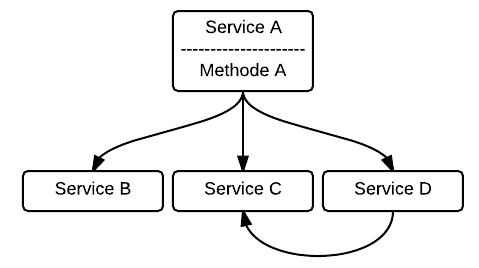
\includegraphics[scale=0.35]{flow.png}
 	\caption{SOMAD call graph.}
    \label{fig:flow}
\end{figure}

In this hypothetical example, SOMAD will likely detect Service A as a Tiny Service as it only has one method and its highly coupled with other services to complete its abstraction. 

As a summary, the outcomes of this first step are reverse engineered SOAs given as a multi-oriented graph and a list of services suspected to be involved in antipatterns.

\subsection{Re-orchestrate services}

In this step we aim to re-orchestrate the services calls in order to reduce the antipatterns detected by SOMAD in the previous step. To do so, we first select the goals we want to reach in the original targeted system and construct a multiple orienteering problem that will serve as heuristic for our planner. Next, we construct a planning problem using the outputs of the step 1 and we formalize it using the PDDL (Planning Domain Definition Language). Finally, we submit this problem to the LAMA \cite{richter2010lama} planer and forward the generated plan to SOMAD in order to assess its quality. In what follows, we will describe each process of this step in details.

\subsubsection{Selecting Goals: }Martin Fowler wrote in his best-seller \cite{Fowler1999} that refactoring refers “to a change made to the internal structure of software to make it easier to understand and cheaper to modify without changing its observable behavior”. Consequently, we want to be able to re-orchestrate the service without modifying the initial behavior of the targeted system. To achieve this, we want our plan to execute all of the methods executed by the SBS’s before its re-orchestration. We can think of this as a SOA version of the traveling salesman problem where the city are services, districts of city correspond to methods of service and roads between cities and districts are the link found by SOMAD. The targeted system, before refactoring, visits all the city and required district but does it in a sub optimum way while after refactoring, it still visits all the cities but by walking the shortest path. 

\subsubsection{Planing Heuristic: } In order to guide our planer towards the sequence of actions requiring the less time and providing the best quality, we use the solution of an orienteering problem where each node is a service and contains a set of sub-nodes accessible only by him and representing its methods. We construct this problem based on the actions pre-conditions and effects detected by SOMAD during the architecture reverse-engineering performed via the execution traces. The cost to travel from a service A to a service B corresponds to the initialization time of Service B and the cost to go from a service node to a method node corresponds to the execution time of the said method. The cost to travel back from the callee service to the caller is 0 and isn't modeled in the following figures for the sake of clarity. Figure \ref{fig:orienteering} represents the orienteering graph constructed using the data provided by SOMAD in the first step. In addition, a reward of 100 has been attributed to $S_b.m_a, S_c.m_a, S_d.m_a$ and a reward of 80 for $S_a.m_a$. The reward of a method is reduced by 20 for each antipattern the service exposing this method is suspected to participate in. 

\begin{figure}
    \centering
	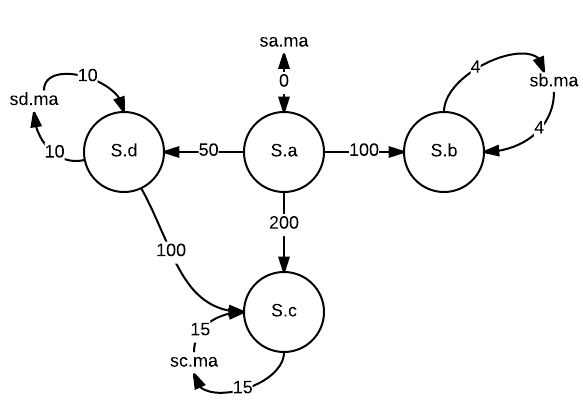
\includegraphics[scale=0.4]{orienteering.png}
 	\caption{Orienteering problem.}
    \label{fig:orienteering}
\end{figure}


While the solution of this generated orienteering problem could constitute a viable heuristic for our planner, it doesn't take advantage of one intrinsic characteristic of SBS’s. To be able to consume a service, we need to build a reference to that service and our experiments showed that the first call to a service -- where the reference is constructed --  construct reference is twice as expensive as the following ones. In other words, if the Service A calls  the Service B; the first time it will cost 100ms will and the second time only 50. To reflect this in our orienteering problem, we construct a multiple orienteering problem where the (simple) orienteering problem is cloned in as many dimension as ordering. We can travel through dimensions via costless edges connecting cloned nodes in each dimension as shown in Figure \ref{fig:multiple_orienteering}. where the cost to go from Sa to Sb has been divided by two, implying that A owns a reference to B in the lower dimension. 
The solution of the multiple orienteering problem will be an ordered list of node and sub-nodes to explore in order to visit them all while minimizing the time needed to do so and maximizing the rewards harvested. 

\begin{figure}
    \centering
	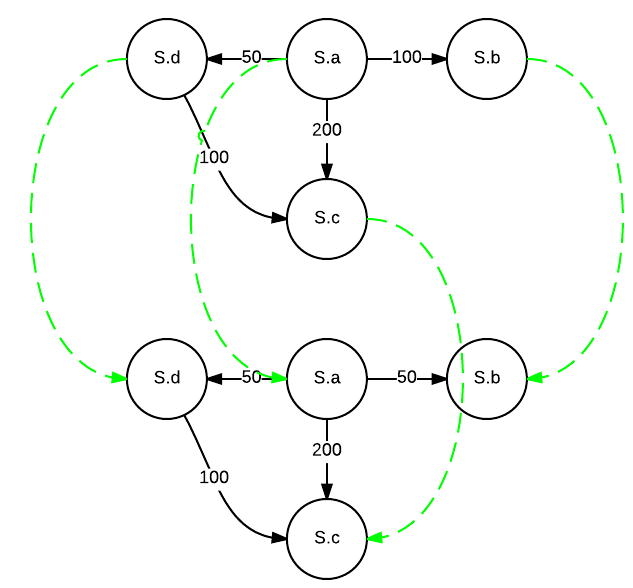
\includegraphics[scale=0.35]{multiple_orienteering.png}
 	\caption{Multiple Orienteering problem.}
    \label{fig:multiple_orienteering}
\end{figure}

\subsubsection{Planning: } In this step, we construct a planning problem using the PDDL and we forward it to the LAMA planner \cite{richter2010lama} which is an evolution of the Fast-Downward planner \cite{helmert2006fast} and has won many prices on several IPC (International Planning Competition). The LAMA planner extends the planning process we discussed in Section III.B in three main ways.
\\ \\
\textit{Landmarks}: The first improvement of LAMA over Fast-Downward is to replace its causal graph heuristic with fast forward based heuristic proposed in \cite{hoffmann2011ff} and combine it with landmarks heuristics. Landmarks have been successfully used by Porteous et al. \cite{porteous2001extraction} and are propositional formulas that must be true in every generated plan for a given task. In order to speed-up the plan generation and find the shortest solution, LAMA directs its search towards states containing many true landmarks \cite{richter2008landmarks}.
\\ \\
\textit{Action costs}: In classical planning, actions don't have cost and execute themselves in discrete time. However, when solving real world problems, actions need to be considered with their costs and required time to be completed. LAMA adapts the heuristics so they use the time and the cost of actions. In our case, actions represent services’ methods calls and they take time; however they don't consume any finite resource. Consequently, we use the solution of the orienteering problem from the previous step as a baseline for the cost of actions. As an hypothetical example, if we have the following ordered list of actions $(a0, a1, ..., a10)$ as solution of the multiple orienteering problem, we will assign them the following cost $(0, 1, ..., 10)$ so the LAMA planner will execute the actions with the higher cost as a last resort to reach a valid plan. 
\\ \\
\textit{Anytime Search}: When LAMA reaches a solution to the planning problem, it continues to search for the best solution by using successive weighted A* graphs. Each iteration sees the weights of A* edges to be decrease and this process runs until resources or time become exhausted. In our case, finding optimal plan is not enough as this plan will be the best in terms of time and resources consumption but not in terms of antipatterns. Consequently, we allow LAMA only a few iterations and stop the anytime search as soon as the improvement starts to lower and forward the current plan to final step of SOMAD-R.

\subsection{Generation of mockup traces}

The output of the planning step is a set of executable actions; however, we still don't have assessed the quality of the newly generated solution. Indeed, only SOMAD knows how to compute the quality of the solution. Consequently, we need to generate a SOMAD understandable input that reflects the current solution. To do so, we generate mockup execution traces based on our current plan. For each action of the solution, a in and out traces are generated as same as a timestamp based on the real ones. For example, if the generated solution ordered calls such as Service A calls Service D, C and Service B, we will generate the traces presented by Figure \ref{fig:generated_traces}.

\begin{figure}
\scriptsize{192.168.1.1 1372366511048 in ServiceA.Ma        \\          
...192.168.1.1 1372366511436 in ServiceD.Ma \\
......192.168.1.1 1372366511536 in ServiceC.Ma\\
......192.168.1.1 1372366511566 out ServiceC.Ma\\
...192.168.1.1 1372366511586 out ServiceD.Ma\\
...192.168.1.1 1372366511686 in ServiceB.Ma\\
...192.168.1.1 1372366511694 out ServiceB.Ma\\
192.168.1.1 1372366511694 out ServiceA.Ma}\\
 	\caption{Generated execution traces.}
    \label{fig:generated_traces}
\end{figure}


The generated traces are sent back to SOMAD which will assess the quality of the solution in terms of antipatterns. The output of SOMAD will change as the orchestration of services is not the same in the generated solution and antipatterns might have been added / removed. Consequently, the solution to the orienteering problem will generate a different heuristic leading to a different solution. Each solution is saved and we return the most qualitative one when time or resources are exhausted. 

\section{Experimentation}

We perform our experiments on Home-Automation. Home-Automation has been developed independently for controlling remotely many basic household functions for elderly home care support. It includes 13 services with a set of 7 predefined uses-case scenarios. In our experiment, we try to remove as many antipatterns from Home-Automation by using the refactoring capacities of SOMAD-R while preserving the behaviour of the system. 
In this subsection, we discuss the process and results of the refactoring part of SOMAD-R.


\subsection{Methodology}

The creator of Home-Automation published their tool with a set of four test scenarios. In order to have near real-world execution traces we have instrumented Home-Automation as it does not produce qualitative execution traces by default. As Home-Automation is a Service Component Application (SCA, an architectural style on top of SOA) it supports aspect weaving and we leverage this feature to insert or tracing statement or probes. Aspects can be weaved by directly interacting with the running environment of an SCA, fraSCAti for Home-Automation and therefore, avoiding to weave directly the target system or to modify its source code. If neither the source code nor the running environments are accessible, alternatives consist in instrumenting the virtual machine if any, the web server, or the operating system. For example, LTTng \cite{Fournier2009} provides Linux instrumentation with a very low overhead.  

\subsection{Scenario}

One of the four scenarios provided by the development team of Home-Automation consists in retrieving the personal information of a patient and send them to his doctor. The following figure presents the scenario with the services names, the purpose of the services, the instantiation time and the initial orchestration of services. The original orchestration requires 472 ms to complete and contains five different antipatterns.


\begin{itemize}
  \item Multi-Service: IMediator
  \item Chatty-Service: PatientDAO and IMediator
  \item Knot: PatientDAO
  \item BottleNeck: PatientDAO, IMediator
  \item Chain Service : IMediator $\rightarrow$ Communicaton Service $\rightarrow$ PatientDAO $\rightarrow$ PatientDAO\{1,2,4\}
\end{itemize}

Home-Automation may appear to the reader as a poorly build system as all its services are involved in at least one antipattern. However, as explained in length in \cite{ Palma, Nayrolles2013a} Home-Automation has been built for the sole purpose of showing how to use the SCA functionalities of the fraSCAti environment. Consequently, many methods are duplicated or poorly encapsulated in order to showcase the different ways of using fraSCAti capabilities.

\begin{figure}
    \centering
	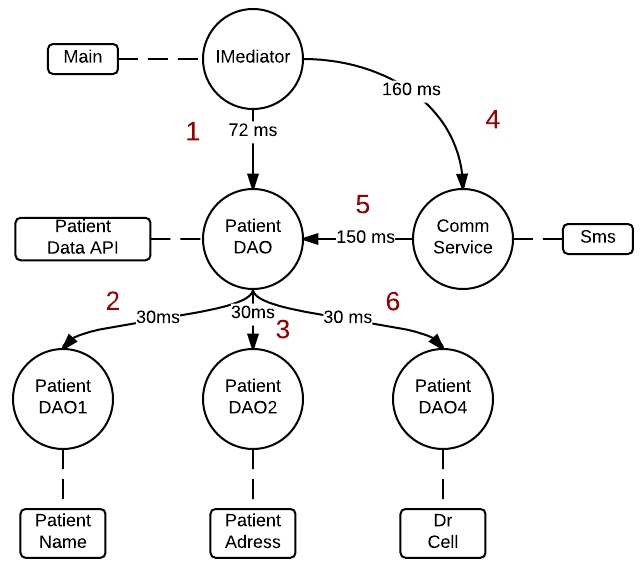
\includegraphics[scale=0.35]{scenario1.png}
 	\caption{HomeAutomation scenario: Send patient information to his doctor (original orchestration).}
    \label{fig:scenario1}
\end{figure}

In order to test the efficiency of our heuristic based on the multiple orienteering problem, we ran the experiment with two different LAMA planners. The first planner uses the original greedy heuristics and the second one uses the heuristic presented in this paper. 

\subsection{Results}

The figures \ref{fig:scenario2} and \ref{fig:scenario3} present the orchestration found by SOMAD-R under LAMA's original heuristic and under our orienteering heuristic, respectively.
In figure \ref{fig:scenario2}, the generated plan requires the services to be consumed in the following order: \textit{IMediator}, \textit{PatientDAO}, \textit{PatientDAO4}, \textit{PatientDAO3}, \textit{PatientDAO1} and \textit{Communication Service} and is able to reach all the required goals in time t = 400 ms (-15\%) while removing the Service chain antipattern which was present in the first orchestration according to SOMAD results.

\begin{figure}
    \centering
	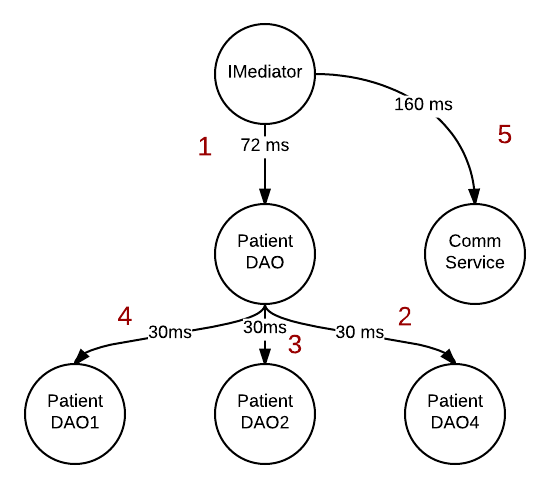
\includegraphics[scale=0.35]{scenario2.png}
 	\caption{HomeAutomation scenario: Send patient information to his doctor (greedy orchestration).}
    \label{fig:scenario2}
\end{figure}

In Figure \ref{fig:scenario3}, the generated plan requires the services to be consumed in the following order: \textit{IMediator}, \textit{Communication Service}, \textit{PatientDAO}, \textit{PatientDAO4}, \textit{PatientDAO3}, \textit{PatientDAO5} in a total of t = 322 ms (-32\%). Furthermore, according to SOMAD's detection, the orienteering based orchestration remove three antipatterns: \textit{The Knot}, \textit{The BottleNeck} and the \textit{MultiService}.  

\begin{figure}
    \centering
	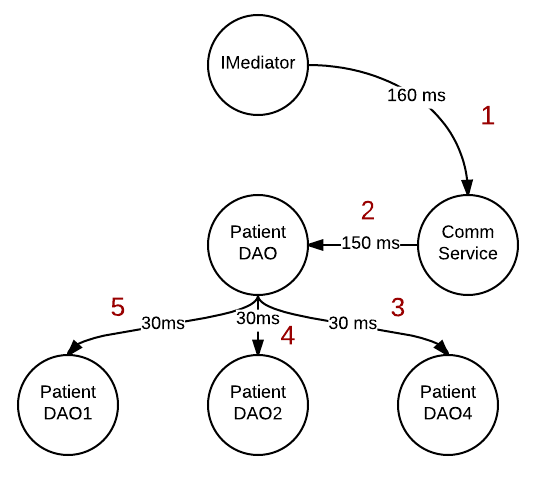
\includegraphics[scale=0.35]{scenario3.png}
 	\caption{HomeAutomation scenario: Send patient information to his doctor (orienteering orchestration).}
    \label{fig:scenario3}
\end{figure}

As a summary, SOMAD-R using the LAMA planner was able to improve the performance of this scenario by 15\% while improving its quality through the removal of three antipatterns. We proved the efficiency of our orienteering heuristic and the relevance of our approach as SOMAD-R is able to improve the performance of the scenario by 32\% while removing a total of three antipatterns when the LAMA planner uses it.

\section{Conclusion \& Future Work}

The refactoring process is a critical life stage of every complex system if we are to ensure the architectural quality of these systems. Nevertheless, the service oriented architecture enables SOAs to be evolved quickly and easily and may allow poor design solution known as SOA antipattern to be inserted. In this paper, we present a novel approach named SOMAD-R which allows the refactoring of SBSs using the SOMAD detection approach and planning techniques. We perform experimentations on HomeAutomation aiming the formal validation of our approach: (i) We refactor the initial system using our approach and reduce the number of SOA Anitpatterns instances from 5 to 2 without loss any functionalities and (ii) we reduce the needed time for its execution by 32\%.
 
As a future work, we shall investigate how to use SOMAD-R for steming the appearance of antipatterns during the development of SBSs. Also, antipatterns are not all dangerous in the same way; therefore, we would like to add, in a near future, a weight to SOA antipattern instead of counting their number and improve our heuristic. 

%
\bibliographystyle{splncs} 
\bibliography{/home/math/Dropbox/writing/library.bib}

\end{document}
